En Guatemala, según datos del Conadi (Consejo Nacional para la Atención de las Personas con Discapacidad) recogidos hasta el mes de marzo del año 2021, existían entre 240,000 y 250,000 personas que utilizaban la lengua de señas como su principal herramienta de comunicación \cite{Conadi2021} . Sin embargo, el uso de esta lengua generaba barreras comunicativas entre una persona oyente y una persona sorda. Estas barreras limitaban la comunicación diaria de estas personas, restringiendo sus oportunidades e independencia.

Esta aplicación tuvo un enfoque especial en las frases de uso diario, preguntas, consultas y dudas que podían surgir en un día cotidiano, ya que estas personas enfrentaban muchos problemas para comunicarse en la realización de tareas cotidianas. Aunque estas tareas podían considerarse triviales para otros, para este sector representaban un reto significativo. Además, se buscó fomentar una mayor autonomía para estas personas, lo que les permitió una inserción más rápida, dinámica y amplia dentro del mundo laboral, facilitando así la obtención de una variedad más amplia de empleos.

También se destacaron las dificultades y barreras de lenguaje que podían ocasionar problemas más serios en situaciones delicadas y de alto estrés. Por ejemplo, en casos en los que las personas que usaban la lengua de señas enfrentaban grandes dificultades para escribir o comunicarse de cualquier otra forma que no fuera mediante esta lengua. Esto podía ocurrir en emergencias médicas, donde la obtención de información básica del paciente era imperativa, o en situaciones como un robo o la necesidad de pedir indicaciones o información bajo estrés, como al interactuar con un agente de policía. Estas son solo algunas de las muchas situaciones en las que las personas que necesitaban la lengua de señas podían encontrarse en una seria desventaja o en riesgo, lo que hacía que una comunicación óptima y la posibilidad de hacer y responder preguntas fueran de gran importancia.

Un aspecto fundamental de este proyecto fue la integración de los diferentes componentes tecnológicos para que trabajaran como una unidad cohesiva en lugar de entidades separadas. Esta integración tuvo una relevancia crítica, ya que permitió desarrollar un sistema que conecta las capacidades de los modelos de inteligencia artificial, la funcionalidad de la aplicación móvil y la infraestructura del servidor. La aplicación tenía como objetivo principal permitir a los usuarios grabar videos de personas utilizando LENSEGUA, enviar textos en español LENSEGUA, y proporcionar herramientas accesibles directamente en sus manos. Para lograr esto, fue indispensable contar con modelos sólidos para el procesamiento de datos, una aplicación intuitiva que sirviera como puente entre los usuarios y la tecnología, y un servidor robusto que facilitara la comunicación entre todos los componentes. Este enfoque integral no solo garantizó la efectividad del sistema, sino que también aseguró su escalabilidad y capacidad para atender las necesidades reales de la comunidad sorda.

\begin{figure}[H]
    \centering
    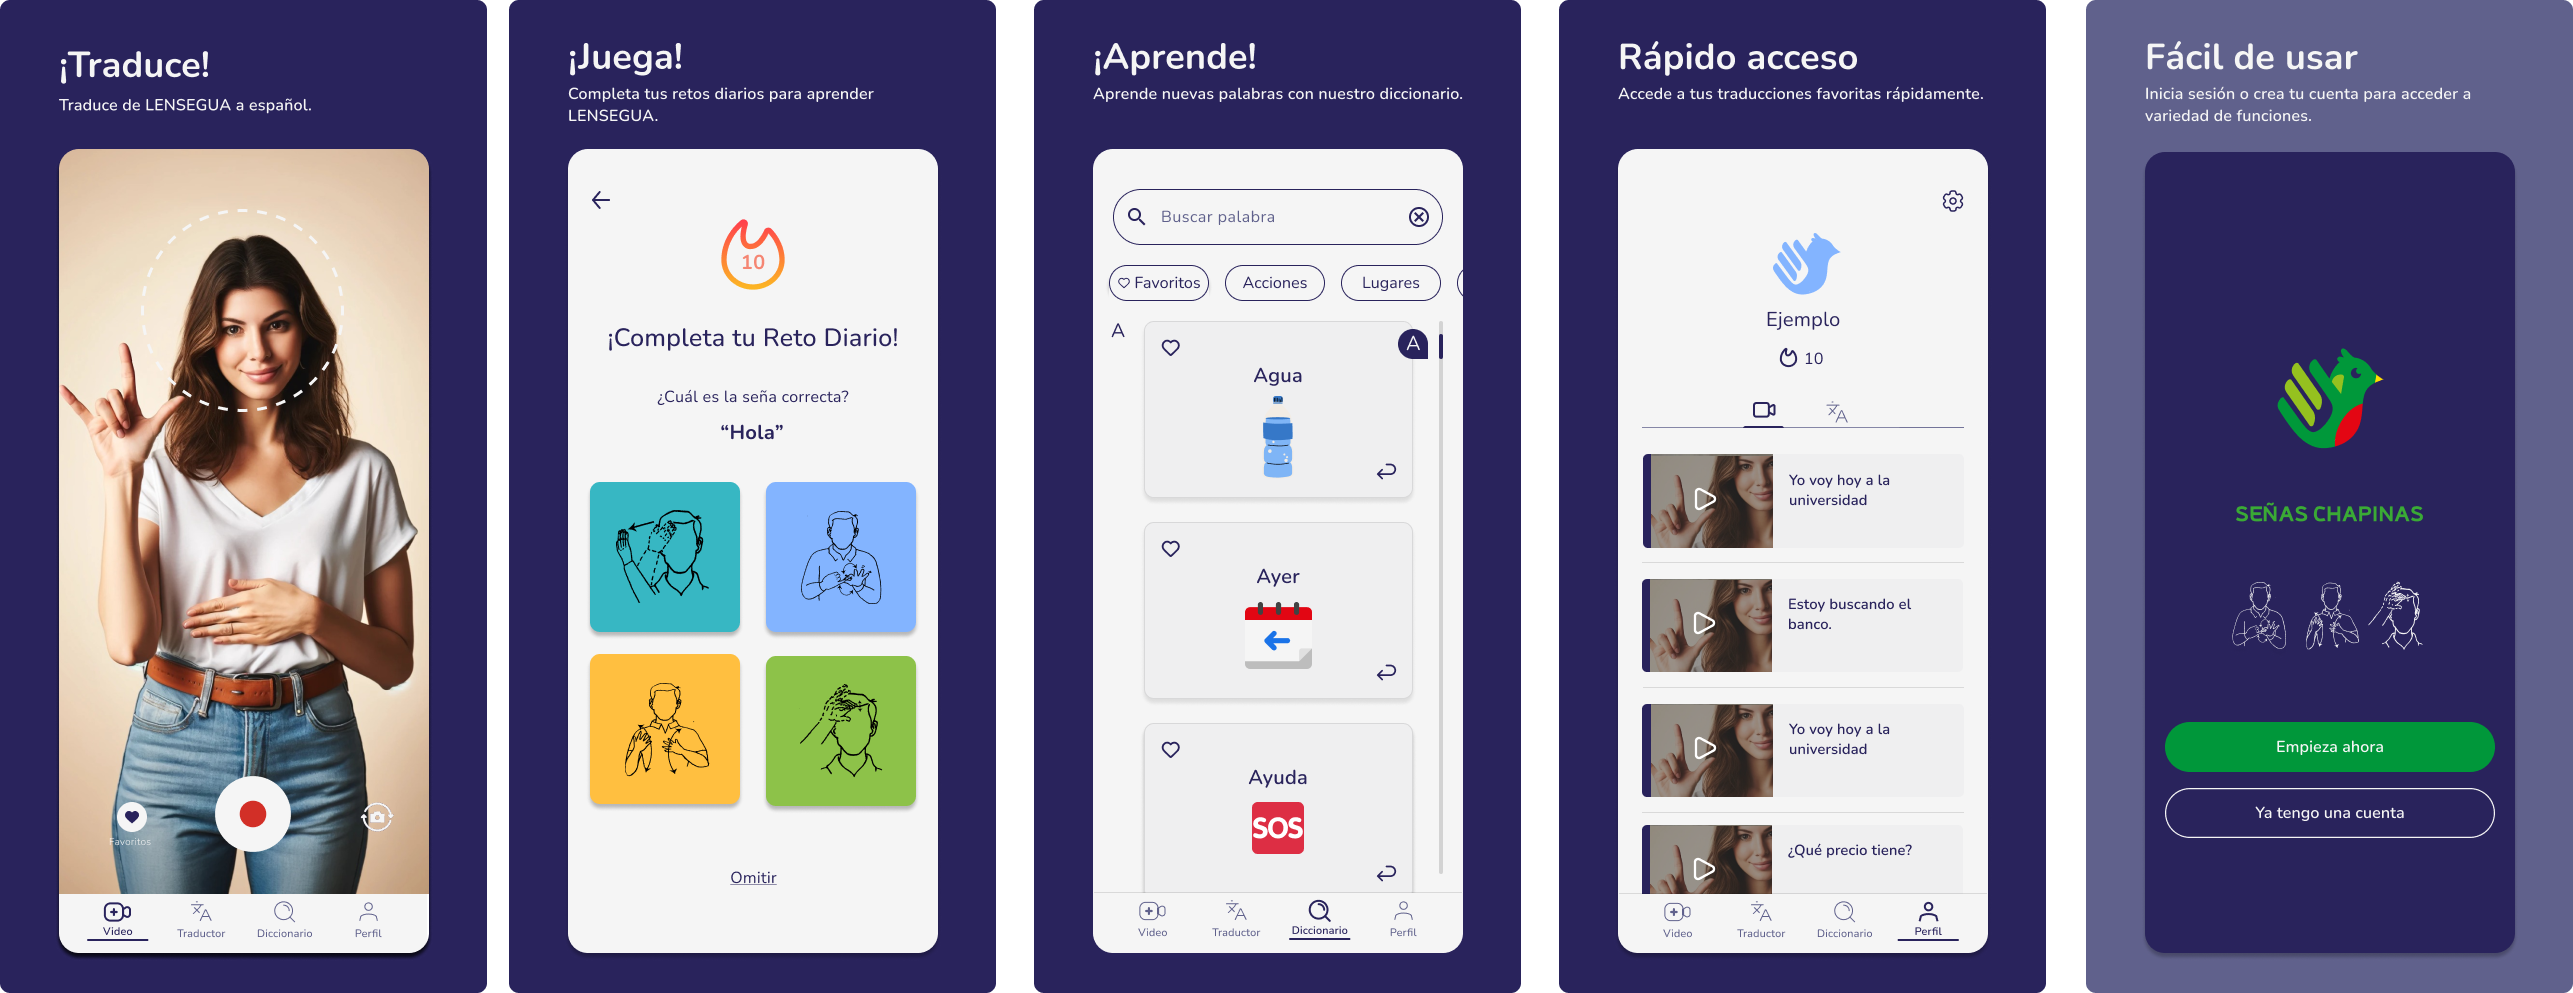
\includegraphics[width=0.5\textwidth]{figuras/capturas_app.png}
    \caption{Aplicación: Señas Chapinas.}
    \label{fig:capturas_app}
\end{figure}